
В настоящей главе формулируются основные понятия, используемые в курсовой работе. Приводится классификация (согласно работе \cite{SI.SIS.SIR}) базовых моделей развития эпидемий. Объясняется принцип построения этих моделей.

%%%%%%%%%%%%%%%%%%%%%%%%%%%%%%%%%%%%%%%%%%%%%%%%%%%%%%%%%%%%%%%%%%%%%%%%%%%%%%%%
\section{Модель. Индекс репродукции}\label{1sec:model.R0}
%%%%%%%%%%%%%%%%%%%%%%%%%%%%%%%%%%%%%%%%%%%%%%%%%%%%%%%%%%%%%%%%%%%%%%%%%%%%%%%%
Существует три основных типа детерминированных моделей инфекционных заболеваний, которые распространяются в популяции при непосредственном контакте человека с человеком. Здесь эти простейшие модели формулируются как начальные задачи для систем обыкновенных дифференциальных уравнений и анализируются математически. Важно понять их поведение, прежде чем рассматривать общие модели, включающие большее количество факторов.\newline
Модель (фр. modèle от лат. modulus «мера, аналог, образец») — система, исследование которой служит средством для получения информации о другой системе\cite{Uemov}; представление некоторого реального процесса, устройства или концепции\cite{SSE.Vocabulary}.
Термином моделирование обозначают как построение (создание) моделей, так и их исследование.
Одним и тем же системам могут быть сопоставлены несколько моделей разных видов. 
  Модели используются для\\
1) идентификации и лучшего понимания систем,\\
2) моделирования поведения систем,\\
3) предсказания их будущего поведения,\\
4) управления системой.\\
Очевидно, что с каждым пунктом задача все усложняется. И хотя конечная цель состоит в том, чтобы контролировать систему, она не всегда достижима.
Рассмотрим простую модель заражения(распространения инфекции)\skip
1-ый шаг: Первый зараженный человек. Будем считать, что в он контактирует с $k$ людьми. И вероятность с которой он заражает каждого из них $p$.\skip
2-ой шаг: Каждый зараженный из 1-ой волны встречает $k$ новых людей и заражает из с вероятностью $p$.\skip
3-ий шаг:...
Население представимо в виде дерева. 
This is Galton-Watson branching stochastic process

$pk$ - среднее число зараженных от одного узла(verage number of secondary infections from one node)
\begin{figure}[h]

\centering

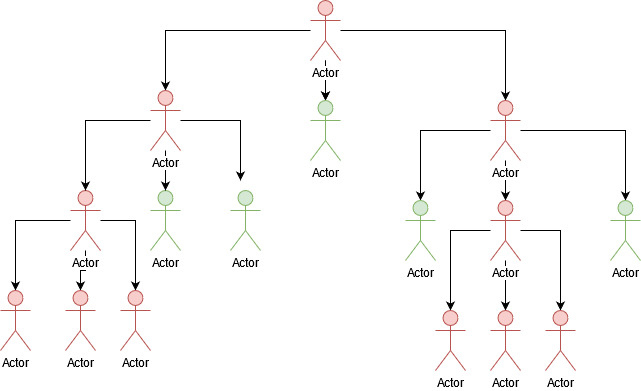
\includegraphics[width=0.8\linewidth]{transmission_schem.jpg}

\caption{Иллюстрация передачи заболевания при k=3 и p=0.(6)}

\label{fig:mpr}

\end{figure}
Число $pk$ настолько важно, что получило собственное название
\begin{equation}
R_0=pk\end{equation}
- индекс репродукции, среднее число вторичных инфекций, возникающих при введении одного инфицированного индивидуума в принимающую популяцию, где все восприимчивы.

На n шаге среднее число инфицированных людей
\begin{equation}
R_0^n= (pk)^n
\end{equation}
Если $R_0 > 1$, индекс репродукции будет расти геометрически, т.к. $R_0^n$.\skip
Если $R_0 < 1$, индекс репродукции будет геометрически убывать.

Когда $ n \rightarrow t $, геометрический рост становится экспоненциальным.
На рисунке ниже приведены индексы репродукции различных вирусных инфекциях.
\begin{figure}[h]

\centering

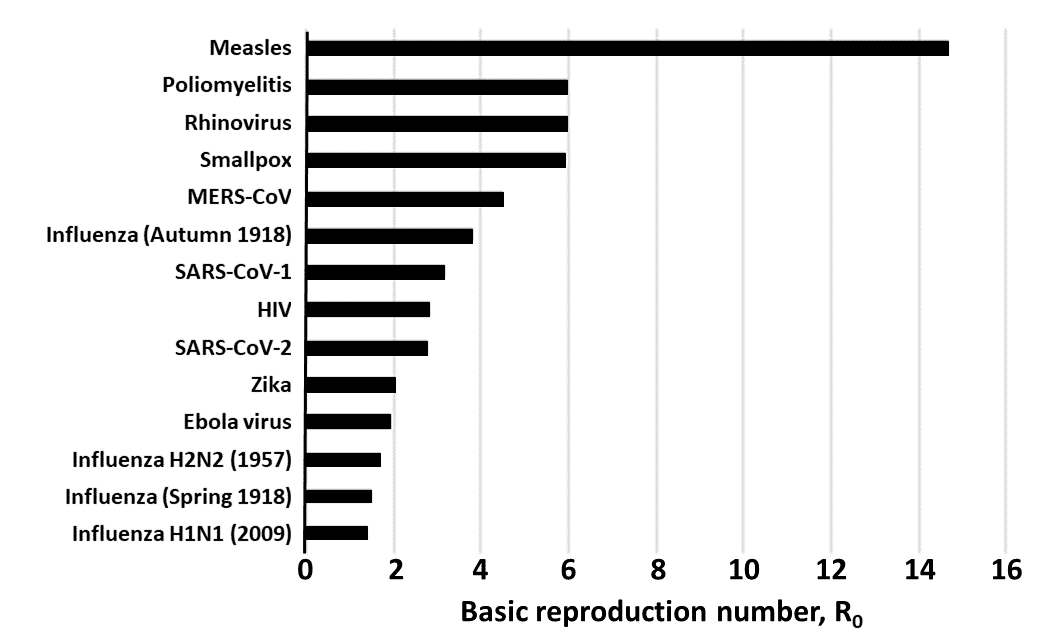
\includegraphics[width=0.8\linewidth]{Basic-reproduction-numbers.png}

\caption{Оценочные значения $R_0$ при различных вирусных инфекциях, полученные из различных опубликованных источников}

\label{fig:mpr}

\end{figure}
Отсюда видно, что повлиять на распространение эпидемии ты можем двумя способами:
\begin{enumerate}
\item снизив вероятность заражения (мыть руки, надевать маски и т. д.),
\item сократив количество встреч с людьми (карантинные меры).
\end{enumerate}

%%%%%%%%%%%%%%%%%%%%%%%%%%%%%%%%%%%%%%%%%%%%%%%%%%%%%%%%%%%%%%%%%%%%%%%%%%%%%%%%
\section{Базовые модели развития эпидемии: SI, SIS, SIR}\label{2sec:basic-models}
%%%%%%%%%%%%%%%%%%%%%%%%%%%%%%%%%%%%%%%%%%%%%%%%%%%%%%%%%%%%%%%%%%%%%%%%%%%%%%%%
Начиная с самых ранних времен моделирования эпидемий, основными элементами описания инфекционных болезней были три эпидемиологических класса Восприимчивые(Susceptible), Инфицированные(Infected) и Выздоровевшие(Removed), которые можно описать как
\begin{itemize}
\item[-] люди, которые здоровы и могут заболеть
\item[-] люди, которые инфицированы и способны распространять болезнь
\item[-] люди, которые переболели и выработали иммунитет(или умерли).
\end{itemize}

Таким образом, базовыми переменными, определяющими состояние населения во время эпидемии, являются:
\begin{itemize}
\item[-] S(t) число восприимчивых в момент времени t;
\item[-] I(t) число инфицированных в момент времени t;
\item[-] R(t) число невосприимчивых в момент времени t;
\end{itemize}

Разумеется, эпидемиологических классов, характеризующих заболевание, может быть больше, но приведенного выше описания вполне достаточно для описания простейших моделей.


\textbf{Рассмотрим модель SI.} Эта аббревиатура происходит от английских слов Susceptible — Infected (Восприимчивые - Инфицированные).

$S \rightarrow I$
\begin{equation} \label{1problem}
    S(t) + I(t) =N
    \end{equation}
$\beta$- скорость передачи/заражения, количество передающих контактов в единицу времени;

$T_c= 1/\beta$- время между передающими контактами

Уравнения заражения:
\begin{equation}
I(t+\delta t) =I(t) +\beta S(t)/N \cdot I(t)\delta t,
$$ $$
\dot{I}=\beta S(t)/N \cdot I(t)
\end{equation}

Переобозначим: $$ i(t) =I(t)/N,$$ $$s(t) =S(t)/N$$
Получим уравнения:
\begin{equation}
    \dot{i(t)}=\beta s(t)i(t)
    $$ $$
    \dot{s(t)}= - \beta s(t)i(t)
    $$ $$
    s(t) +i(t) = 1
    \end{equation}
или, что то же самое, дифференциальное уравнение:
\begin{equation}
    i(t = 0) =i_0
    $$ $$
    \dot{i}=\beta(1 - i(t))i(t)
 \end{equation}
Решение этого уравнения имеет вид:
$$i(t) = i_0/(i_0+ (1 - i_0)e^{-\beta\cdot t} )$$
Предел при $ t \rightarrow \infty $
$$ i(t) \rightarrow 1$$
$$ s(t) \rightarrow 0$$
\begin{figure}[h]

\centering

\includegraphics[width=0.8\linewidth]{SI.fig}

\caption{График модели SI при $beta$=0.7 и начальном числе инфицированных - 1%}

\label{fig:mpr}

\end{figure}



\textbf{Рассмотрим модель SIS.}
Susceptible — Infected - Susceptible (Восприимчивые - Инфицированные - Восприимчивые).

$S \rightarrow I \rightarrow S$
\begin{equation}
    S(t) + I(t) =N
    \end{equation}
$\beta$ - скорость заражения,
$\gamma$ - скорость восстановления;

$T_r= 1/\gamma$- время восстановления

Уравнения заражения:
\begin{equation}
    \dot{i(t)}=\beta s(t)i(t) -\gamma i(t)
    $$ $$
    \dot{s(t)}= - \beta s(t)i(t)+\gamma i(t)
    $$ $$
    s(t) +i(t) = 1
    \end{equation}

Дифференциальное уравнение,  $i(t = 0) =i_0$:
\begin{equation}
    \dot{i(t)}=(\beta- \gamma - i(t))i(t)
 \end{equation}
Решение этого уравнения имеет вид:
$$i(t) = (1-\gamma / \beta )C/(C+e^{-(\beta -\gamma)t}),$$
где $$C = \beta i_0/(\beta - \gamma -\beta i_0)$$
Предел при $ t \rightarrow \infty $
$$ \beta >\gamma , i(t) \rightarrow (1 -\gamma / \beta)$$
$$ \beta < \gamma ,i(t) = i_0 e^{(\beta -\gamma)t} \rightarrow 0$$



\textbf{Рассмотрим модель SIR.}
Susceptible — Infected - Recovered (Восприимчивые - Инфицированные - Выздоровевшие).
Эта модель получила популярность в силу простоты построения и использования. Она позволяет точно моделировать эпидемии гриппа и других заболеваний (где выздоровевшие имеют иммунитет) в больших городах, вводить новые параметры и анализировать разные сценарии.

$S \rightarrow I \rightarrow R$
\begin{equation}
    S(t) + I(t) + R(t) = N
    \end{equation}
$\beta$ - скорость заражения,
$\gamma$ - скорость восстановления;

Уравнения заражения:
\begin{equation}
    \dot{s(t)}= - \beta s(t)i(t)
    $$ $$
    \dot{i(t)}=\beta s(t)i(t) -\gamma i(t)
    $$ $$
    \dot{r(t)} = \gamma i(t)
    $$ $$
    s(t) +i(t) + r(t) = 1
    \end{equation}

Дифференциальное уравнение:
\begin{equation}
    \dot{s}=-\beta s dr/dt 1/\gamma
    $$ $$
    s = s_0 e^(-\beta/\gamma r)
    \dot{r} = \gamma(1-r-s_0 e^{-\beta/\gamma r}
 \end{equation}
Решение этого уравнения имеет вид:
$$ t = 1/\gamma \int_0^r dr/(1-r-s_0 e^{-\beta / \gamma r},$$

Предел при $ t \rightarrow \infty $, $ dr/dt = 0$, $r_\infty = const$,
$$ 1 -r_\infty = s_0 e^{-\beta/\gamma r_\infty}$$
$$ r_\infty = 1- e^{R_0 r_\infty}, R_0 = \beta/\gamma$$
$$(r_\infty)'|_{r_\infty=0} = (1 - e^{-R_0 r_\infty})'|_{r_\infty =0}$$
критическая точка: $R_0 = 1$
$r_\infty$ - общий размер вспышки
Если $R_0 > 1, \beta > \gamma , r_\infty = const>0$, эпидемия имеет место.
Если же $ R_0 < 1, \beta < \gamma , r_\infty \rightarrow 0$
$\beta$ - скорость заражения, $\gamma$ - скорость восстановления $\rightarrow$
Индекс репродукции $R_0 = \beta/\gamma = T_r/T_c$ - это среднее число зараженный человеком людей до его выздоровления
$$R_0 = E[\beta\tau] = \beta \int_0^\infty \gamma\tau e^{-\gamma\tau} d\tau =\beta/\gamma$$
........


%%%%%%%%%%%%%%%%%%%%%%%%%%%%%%%%%%%%%%%%%%%%%%%%%%%%%%%%%%%%%%%%%%%%%%%%%%%%%%%%
\section{Модель SEIR}\label{1sec:SEIR}
%%%%%%%%%%%%%%%%%%%%%%%%%%%%%%%%%%%%%%%%%%%%%%%%%%%%%%%%%%%%%%%%%%%%%%%%%%%%%%%%
Susceptible — Exposed - Infected - Recovered (Восприимчивые - Контактные - Инфицированные - Выздоровевшие).
Под Контактными(Exposed(e)) понимаются зараженные люди, которые не могут распространять болезнь.
По этой модели развиваются по-настоящему опасные эпидемии, поскольку длительный инкубационный период может препятствовать своевременному обнаружению заболевания.

$$S(t) + E(t) + I(t) + R(t) = N$$
\begin{equation*}
    \dot{s} = -(1 - u)\beta si
    $$ $$
    \dot{e} = (1 - u)\beta si -\alpha e
    $$ $$
    \dot{i}= \alpha e - \gamma i
    $$ $$
    \dot{r} = \gamma i
\end{equation*}

где $\alpha$ --- это скорость, с которой индивид переходит из
класса контактных в класс инфецированных, $u$ представляет собой степень социального дистанцирования ($u = 0$ - социальное дистанцирование не применяется, $u = 1$ - полная изоляция) и $ s + e + i + r = 1$


%%%%%%%%%%%%%%%%%%%%%%%%%%%%%%%%%%%%%%%%%%%%%%%%%%%%%%%%%%%%%%%%%%%%%%%%%%%%%%%%
\section{Модель SIDARTHE}\label{1sec:SIDARTHE}
%%%%%%%%%%%%%%%%%%%%%%%%%%%%%%%%%%%%%%%%%%%%%%%%%%%%%%%%%%%%%%%%%%%%%%%%%%%%%%%%

В модели SIDARTHE популяция разделена на следующие 8 состояний: \newline
 S, Восприимчивые (Susceptible); \newline
 I, Инфицированные (Infected) (бессимптомные больные, необнаруженные); \newline
 D, Диагностированные (Diagnosed) (бессимптомные больные, обнаруженные);  \newline
 A, Больные (Ailing) (болеющие с симптомами, необнаруженные);  \newline
 R, Распознанные (Recognised) (больные с симптомами, обнаруженные); \newline
 T, Threatened (зараженный с угрожающими жизни симптомами, обнаруженный);  \newline
 H,  Выздоровевший (Healed); \newline
 E, Исчезнувший (Extinct) (умерший). \newline

\begin{equation*}
    \dot{S(t)} = -S(t)(\alpha I(t)+\beta D(t) +\gamma A(t) + \delta R(t))
  \end{equation*}
  \begin{equation*}
   \dot{I(t)} = S(t)(\alpha I(t) + \beta D(t) +\gamma A(t) +\delta R(t) -(\epsilon+\zeta+\lambda)I(t)
\end{equation*}
\begin{equation*}
    \dot{D(t)} = \epsilon I(t) - (\eta +\rho)D(t)
\end{equation*}
\begin{equation*}
    \dot{A(t)} = \zeta I(t) - (\theta+\mu+\kappa)A(t)
  \end{equation*}
  \begin{equation*}
    \dot{R(t)} = \eta D(t) + \theta A(t) - (\nu+\xi) R(t)
    \end{equation*}
    \begin{equation*}
    \dot{T(t)} =\mu A(t) + \nu R(t) - (\sigma+\tau) T(t)
    \end{equation*}
  \begin{equation*}
    \dot{H(t)} =\lambda I(t) +\rho D(t) +\kappa A(t) +\xi R(t)  +\sigma T(t)
    \end{equation*}
 \begin{equation*}
    \dot{E(t)} = \tau T(t)
\end{equation*}

где большие латинские буквы обозначают состояния популяции,а все рассматриваемые параметры, обозначаемые греческими буквами, являются положительными числами. В частности парметры:
\begin{itemize}
\item $\alpha, \beta, \gamma, \delta$ соответственно обозначают скорость передачи (то есть вероятность передачи болезни в одном контакте, умноженную на среднее число контактов на человека), обусловленную контактами между Восприимчивым субъектом и Инфицированным, Диагностированным, Больным, Распознанным субъектом. Как правило,$\alpha$ больше, чем $\gamma$(предполагая, что люди стараются избегать контактов с субъектами, проявляющими симптомы, даже если диагноз еще не был поставлен), что, в свою очередь, вероятно, больше, чем $\beta$ и $\delta$ (предполагая, что субъекты, которым был поставлен диагноз, должным образом изолированы).Эти параметры могут быть изменены политикой социального дистанцирования (например, закрытие школ, удаленная работа и т. д.). Риск заражения из-за субъектов с угрожающими жизни симптомами, лечащихся в соответствующих отделениях интенсивной терапии, считается незначительным.
\item $\epsilon, \theta$ коэффициент вероятности обнаружения относительно бессимптомных и симптоматических случаев соответственно. Эти параметры, также поддающиеся модификации, отражают уровень внимания к заболеванию и количество тестов, проведенных в популяции. Обратите внимание , что $\theta$ обычно больше, чем $\epsilon$, так как люди с симптомами с большей вероятностью пройдут тестирование.
\item $\zeta$ и $\eta$ обозначим вероятность того, что у инфицированного субъекта, соответственно не знающего и знающего о том, что он заражен, развиваются клинически значимые симптомы, которые, вероятно, сопоставимы. Эти параметры зависят от заболевания и вряд ли поддаются модификации
\item $\mu$ и $\nu$ обозначают скорость, с которой у необнаруженных и обнаруженных инфицированных субъектов развиваются угрожающие жизни симптомы, и, вероятно, они будут сопоставимы, если нет известного специфического лечения, эффективного против болезни, в противном случае, $\mu$ скорее всего будет больше. Эти параметры могут быть снижены с помощью улучшенной медицины и приобретения иммунитета против вируса
\item $\tau$ обозначает уровень смертности (для инфицированных субъектов с угрожающими жизни симптомами) и может быть снижен с помощью улучшенной медицины.
\item $\lambda, \kappa, \xi, \rho$ и $\sigma$ обозначают скорость выздоровления для пяти классов инфицированных субъектов и могут существенно различаться, если соответствующее лечение заболевания известно и принято у диагностированных пациентов, в то время как в противном случае, вероятно, они сопоставимы. Эти параметры могут быть увеличены благодаря усовершенствованным методам лечения и приобретению иммунитета против вируса
\end{itemize}
Мы опускаем вероятность того, что индивид снова станет восприимчивым после того,как уже выздоровел от инфекции, поскольку значение вероятности кажется незначительным (хотя и не нулевым), основываясь на ранних данных \cite{RecoveredTests}\cite{AsymptomaticCarrierTransmission}

\bigskip

Каждая глава завершается краткими выводами. Разумный способ написания выводов --- переписать (это значит использовать те же мысли, но не копировать фразы!) в утвердительной форме (рассмотрено, получено и т.д.) то, что написано во врезке. 
